\documentclass[a4paper,12pt]{article}

\usepackage[T1]{fontenc}
\usepackage[polish]{babel}
\usepackage[utf8]{inputenc}
\usepackage{geometry}
\usepackage{booktabs}
\usepackage{graphicx}
\usepackage{amsmath}
\usepackage{hyperref}
\usepackage{float}

\geometry{left=2.5cm, right=2.5cm, top=2.5cm, bottom=2.5cm}

\title{\textbf{Raport techniczny: Symulacja balistyki wewnętrznej silników rakietowych}}

\author{Paweł Mikołajewski\\Analiza porównawcza systemów napędowych}

\date{\today}

\begin{document}

\maketitle
\newpage

\tableofcontents
\newpage

\section{Wstęp}

Celem niniejszego opracowania jest analiza porównawcza profilów ciągu czterech typów silników rakietowych: dwóch zasilanych paliwem stałym (KNSB oraz APCP) oraz dwóch hybrydowych (N2O z parafiną oraz N2O z HTPB). Wykorzystano modele matematyczne oparte na numerycznym rozwiązywaniu równań balistyki wewnętrznej.

Głównym założeniem przeprowadzonych analiz było porównanie różnych konfiguracji paliwowych przy zachowaniu zbliżonego poziomu całkowitego impulsu silnika, wynoszącego około 3000 Ns. Takie podejście umożliwia ocenę wpływu rodzaju paliwa i architektury układu napędowego na charakterystykę ciągu, czas pracy, wymagania konstrukcyjne oraz zastosowania rakiety bez dominującego wpływu całkowitej energii układu.

Przedstawione wyniki mają charakter porównawczy i służą ocenie zachowania poszczególnych układów napędowych przy zbliżonych wymaganiach energetycznych.

\section{Metodologia i założenia modelowe}

W celu wykonania symulacji przyjęto szereg uproszczeń, które pozwalają na modelowanie zjawisk fizycznych przy zachowaniu efektywności obliczeniowej.

\subsection{Analiza fizyczna i weryfikacja modelu}

Zastosowany model matematyczny obejmuje:

\begin{itemize}

    \item \textbf{Dynamiczny bilans masy i energii:} Równanie różniczkowe dla ciśnienia komory spalania ($P_c$) uwzględnia sprzężenie między generacją gazów a ich wypływem przez dyszę.

    \item \textbf{Modelowanie zapłonu:} Funkcja wykładnicza zapewnia realistyczne narastanie ciśnienia podczas startu.

    \item \textbf{Sprzężenie w silnikach hybrydowych:} Dynamiczna zmiana stosunku O/F oraz wpływ na $C^*$.

    \item \textbf{Ewolucja geometrii:} Aktualizacja powierzchni spalania i objętości komory w czasie.

\end{itemize}

\subsection{Uproszczenia modelu}

\begin{itemize}

    \item Stałe $C^*$ dla każdego paliwa.
    \item Uproszczona geometria ziarna paliwa.
    \item Prawo Marxmana dla regresji paliwa.
    \item Stałe ciśnienie atmosferyczne.
    \item Stały wykładnik adiabaty $\gamma$.

\end{itemize}

\section{Wyniki symulacji}
\begin{figure}[H]
    \centering
    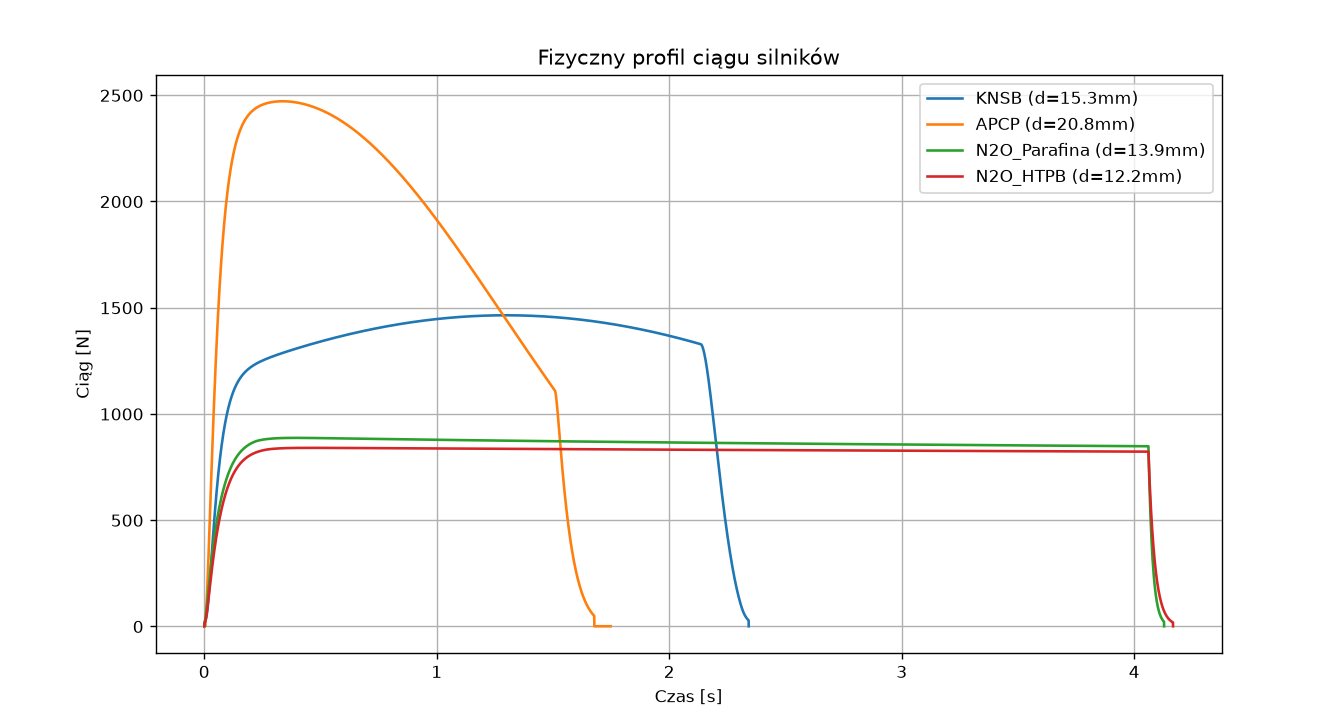
\includegraphics[width=0.9\textwidth]{aa.png}
    \caption{Porównanie przebiegów ciągu dla analizowanych silników rakietowych}
    \label{fig:ciag_porownanie}
\end{figure}
\begin{table}[H]
\centering
\caption{Zestawienie parametrów konstrukcyjnych i osiągów}
\vspace{0.2cm}

\begin{tabular}{lcccc}
\toprule
\textbf{Silnik} & \textbf{Masa paliwa [kg]} & \textbf{Impuls [Ns]} & \textbf{Śr. dyszy [mm]} & \textbf{Czas pracy [s]} \\
\midrule
KNSB & 2.446 & 2999.22 & 15.29 & ok. 2.2 \\
APCP & 1.456 & 3023.65 & 20.81 & ok. 1.6 \\
N2O\_Parafina & 1.699 & 3476.77 & 13.87 & ok. 4.0 \\
N2O\_HTPB & 1.529 & 3339.79 & 12.20 & ok. 4.1 \\
\bottomrule
\end{tabular}

\end{table}

\section{Analiza wyników}

\subsection{Charakterystyka paliw stałych}

APCP wykazuje bardzo wysoki, krótki impuls, natomiast KNSB charakteryzuje się bardziej łagodnym przebiegiem spalania.

\subsection{Charakterystyka silników hybrydowych}

Silniki hybrydowe zapewniają dłuższy czas pracy oraz bardziej stabilny profil ciągu.

\section{Wnioski końcowe}

Przeprowadzona analiza umożliwiła porównanie czterech konfiguracji napędowych przy założeniu impulsu około 3000 Ns.

\begin{enumerate}

\item \textbf{Efektywność energetyczna}

Silniki hybrydowe osiągają wyższą efektywność wykorzystania materiałów pędnych oraz dłuższy czas pracy przy porównywalnym impulsie całkowitym.

\item \textbf{Profil ciągu}

APCP generuje wysoki ciąg początkowy, KNSB zapewnia łagodny przebieg, a hybrydy dają najbardziej stabilny profil.

\item \textbf{Geometria spalania}

Zmiana powierzchni spalania i stosunku O/F istotnie wpływa na charakterystykę pracy silnika.

\item \textbf{Wymagania konstrukcyjne}

APCP wymaga największych średnic dysz i największej odporności termicznej konstrukcji.

\item \textbf{Bezpieczeństwo}

Silniki hybrydowe są bezpieczniejsze dzięki separacji paliwa i utleniacza.

\item \textbf{Założenie projektowe 3000 Ns}

Porównanie wykonano przy zbliżonym impulsie całkowitym 3000 Ns, co pozwala ocenić realny wpływ rodzaju paliwa na przebieg pracy silnika niezależnie od całkowitej energii układu.

\end{enumerate}

\section{Kierunki dalszych prac}

Dalszy rozwój modelu obejmuje:

\begin{itemize}

\item zmienny model $C^*$ zależny od ciśnienia i składu gazów,
\item integrację z NASA CEA,
\item rozbudowę geometrii ziarna paliwa,
\item model erozyjnego spalania,
\item model zbiornika N$_2$O,
\item straty cieplne i model termiczny,
\item analizę wrażliwości parametrów,
\item walidację eksperymentalną,
\item integrację z symulatorem lotu 6-DOF.

\end{itemize}

Docelowo system ma umożliwiać optymalizację paliw dla silników o impulsie około 3000 Ns oraz budowę bazy danych konfiguracji napędowych.
% --- BIBLIOGRAFIA ---
\begin{thebibliography}{9}
\bibitem{Sutton} 
Sutton, G. P., Biblarz, O. (2016). \textit{Rocket Propulsion Elements}. Wiley. 
\bibitem{Marxman} 
Marxman, G. A., Woolridge, C. E., Muzzy, R. J. (1964). \textit{Fundamentals of Hybrid Rocket Combustion}. 
\bibitem{Huzel} 
Huzel, D. K., Huang, D. H. (1992). \textit{Modern Engineering for Design of Liquid-Propellant Rocket Engines}.
\end{thebibliography}
\end{document}